\begin{frame}
    \frametitle{Konzept}
    \framesubtitle{Ausrichtung}
    \begin{columns}
        \begin{column}{0.4\textwidth}
            \begin{block}{Ausrichtung}
                \begin{itemize}
                    \item Drehung
                    \item Getriebe
                    \item Schrittmotor
                \end{itemize}
            \end{block}
        \end{column}
        \begin{column}{0.6\textwidth}
            \centering
            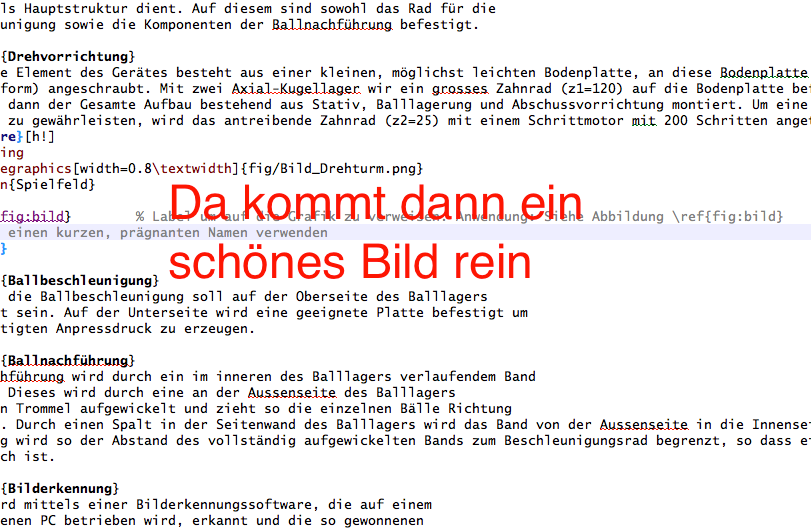
\includegraphics[width=1.0\textwidth, trim = 25mm 23mm 5mm 15mm, clip]{../doc/fig/Bild_Drehturm.png}
        \end{column}
    \end{columns}
\end{frame}

